\documentclass[main.tex]{subfiles}

\begin{document}
Precision measurements at low energy can compete with high energy measurements.

\section{New Physics Searches}
Testing the standard model is important.
There are generaly two ways to experimentally do this.
One is to look for new particles with high energy experiments. 
The other is to look at lower energy experiments very percisely.
The direct detection of new particles is very general and a powerful technique.
Precision measurements, on the other hand, are much more specialized.
Precision measurements are sensitive to only certain channels of new physics.

\section{Beta Decay}
Beta decay is one of the processes by which unstable nuclei lose energy.
The general process is shown in equation \ref{eq:betadecay}

\begin{equation}
	\label{eq:betadecay}
	^{A}_{Z}P \rightarrow ^{A}_{Z\pm 1}D + e^{\pm} + \nu_{e}
\end{equation}

with $^{A}_{Z}P$ being the parent nucleus, $^{A}_{Z \pm 1}D$ being the daughter nucleus, $e^{\pm}$ is the outgoing electron or positron, and $\nu$ is an outgoing neutrino.
The neutrino is an anti-electron neutrino in the case of beta$^{-}$ decay, and an electron neutrino in the case of beta$^{+}$ decay. 
There is also the process of electron capture, where a proton in the nucleus captures an inner electron and turns into a neutron.

The simplist type of nuclear beta decay is allowed beta decay.
There are two types of allowed beta decay, which differ in angular momentum $J$ and isospin $T$ selectrion rules.
The two types are called Fermi and Gamow-Teller beta decay. 
Neither of these transitions change parity.
The difference is that, in a Fermi transition, the change of the angular momentum $J$ and the change of the isospin $T$ is both zero.
For a Gamow-Teller transition, the change in the angular moment $J$ is $0$ or $\pm1$ and the change of the isospin $T$ is $0$ or $\pm 1$.
However, a Gamow-Teller transition cannot cause a transition between two states of $J = 0$. 
These are called superallowed beta decays.
There are also mixed allowed transitions, where both matrix elements of Fermi decay and Gammow Teller decay contribute.
In order to see what physics beyond the standard model beta decay measurements are sensitive to, a closer look at beta decay is needed.

\subsection{Microscopic View of Beta Decay}
At a microscopic level, the process of beta decay involves one of the quarks inside the nucleon emitting a $W$ particle.
This quark changes flavor, and the nucleon changes as well. 
The microscopic view of beta decay (for the beta$^{-}$ case) is shown in figure \ref{fig:betadecaymicro}.

\begin{figure}[!htb]
	\centerline{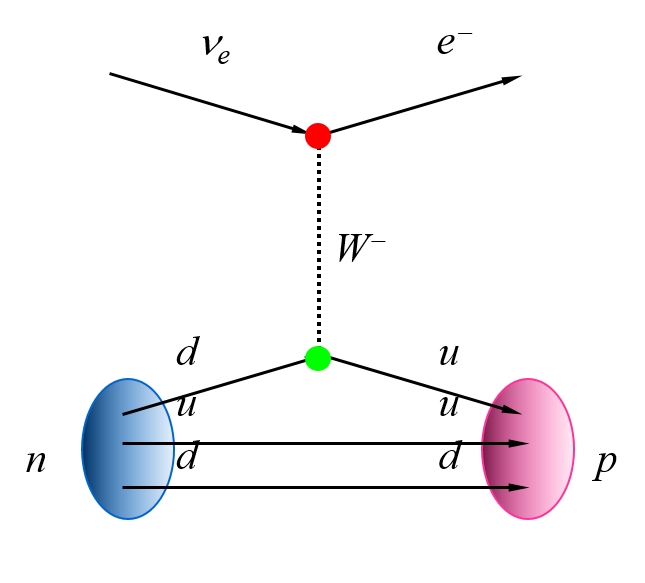
\includegraphics[width=0.5\textwidth]{fig_betadecayzoomedin.png}}
	\caption{What beta$^{-}$ decay looks like microscopically}
	\label{fig:betadecaymicro}
\end{figure}

A down quark in a neutron goest to an up quark.
This process emits a $W^{-}$ boson that decays into an electron and an anti-electron neutrino.
This means that any beta decay measurements are probing the weak sector. 
These measurements are complimentary to high energy measurements of weak interactions.
For this work, a nucleon level treatment of beta decay will suffice.  

\subsection{Matrix elements of Beta Decay}
In order to cacluate the beta decay rate, Fermi's golden rule is needed.
This is shown in equation \ref{eq:fgr}.

\begin{equation}
	\lambda = \frac{2\pi}{\hbar}\|M\|^{2}\rho(E)
	\label{eq:fgr}
\end{equation}

The density of states, $\rho(E)$, will be discusses further in the thesis. 

This matrix element $M$, to first order, is shown in equation \ref{eq:decayrate} \cite{Gon19}

\begin{equation}
	|M|^{2} = \xi [1 + a \frac{\vec{p_{e}} \cdot \vec{p_{\nu}}} {E_{e} E_{\nu}}  +  b \frac{m_{e}}{E_{e}} + \frac{\vec{<J>}}{J} \cdot (A \frac{ \vec{p_{e}} }{E_{e}} + B \frac{\vec{p_{\nu}}}{E_{\nu}} + D \frac{\vec{p_{e}} \times \vec{p_{\nu}}}{E_{e} E_{\nu}})]
	\label{eq:decayrate}
\end{equation}

$\xi$ is written out in equation \ref{eq:xiwrittenout}. 
This equation is written out to linear order.
 
\begin{equation}
	\xi = \frac{1}{2} |M_{F}|^{2} |C_{V} + C'_{V}|^{2} (1 + |\rho|^{2})
	\label{eq:xiwrittenout}
\end{equation}
For equation \ref{eq:xiwrittenout}, $M_{F}$ is the Fermi matrix element, $C_{V}$ and $C_{V}$ are vector coupling constants, and $|\rho|$ is the ratio of the Gamow-Teller matrix element to the Fermi matrix element.
\cite{Gon19}

Going back to equation \ref{eq:decayrate}, $<\vec{J}>$ is the average total angular momentum. 
The constants $a$, $b$, $A$, $B$, and $D$ can be written in terms of the coupling constants as well.
$a$ depends on the ratio of the Fermi and Gamow-Teller matrix elements $\rho$.
This form of the observables informs the experimental design. 

\subsection{Types of Percision Measurements in Beta Decay}
Given the form of equation \ref{eq:decayrate}, to get at different terms, different types of experiments are needed.
A polarized nucleus is need to extract $a$. 
The nuclear spin points in one direction. 
Then, by angular momentum conservation, $\vec{p_{e}} \cdot \vec{p_{\nu}}$ can be found.
Other correlations between energy and momenta have sensitivity to other terms in equation \ref{eq:decayrate}.
Equation \ref{eq:decayrate} is not complete, and many other terms exist. 

For an unpolarized beam where only the energy of the electron is measured, the momenta are averaged over and all terms disappear expect for $b$.
This term is known as the Fierz term, and a measurement of the Fierz term was the ultimate goal of this experiment. 

\subsubsection{Fierz Term}
The Fierz term, $b$, in equation \ref{eq:decayrate}, can be rewritten in terms of effective couplings.
This is shown in equation \ref{eq:bwrittenout}

\begin{equation}
	b =  \pm \sqrt{1 - \alpha^{2}{Z^{2}}}\frac{1}{1 + \rho}Re(\frac{C_{S} + C_{S}'}{C_{V} + C_{V}'} + |\rho|^{2}\frac{C_{T} + C_{T}'}{C_{A} + C_{A}'})
	\label{eq:bwrittenout}
\end{equation}

where $\rho$ is the ratio of the Gamow-Teller matrix element to Fermi matrix element, $\alpha$ is the QED fine structure constant \cite{Gon19}
The subscripts of $C$ indicate which object the coupling corresponds to. 
Here, $A$ means axial vector, $V$ stands for polar vector, $S$ stands for scalar, and $T$ stands for tensor. 
The $C$ coefficients correspond to parity conserving interactions, and the $C'$ coefficents correspond to parity non-conserving coefficents \cite{Lee56}
This means, that in a pure Fermi decay, the Fierz term is sensitive to any non-standard scalar term, while in a pure Gamow-Teller decay, the Fierz term is sensitive to any non-standard Tensor terms. 

The Fermi decays have been measured using super-allowed beta decays.
For most of these measurements, however, decay of interest happens very rarely.
The $ft$ value was measured.
$ft$ values give the value of the Fierz term averaged over the beta decay energy spectrum.
Several measurements of different decays are needed to get a good constraint.
The other part of the Fierz term is the tensor coupling. 
In order to get a good measurement of  tensor couplings, an allowed Gamow-Teller decay must be used. 
In this measurement, the nucleus of interest was $^{20}$F.
 

\end{document}
